\graphicspath{ {./workaround/pictures/} }
\section{Workarounds}
\subsection{Still connection error after press reset button}
If you run the flash command and you got a Timed Out
\begin{lstlisting}
$ idf.py -p /dev/ttyUSB0 flash
Executing action: flash
...
esptool.py v3.3-dev
Serial port /dev/ttyUSB0
Connecting..................
...

A fatal error occurred: Failed to connect to ESP32: Timed out waiting for packet header
$
\end{lstlisting}
you should check if you have problems with the 5V output on your FTDI-board. If yes, you should modify your setup by an external power supply on the 5V pin on the board (see \ref{ESP32-S-CAM-setup-with-external-5v}).

\begin{figure}[H]
\centering
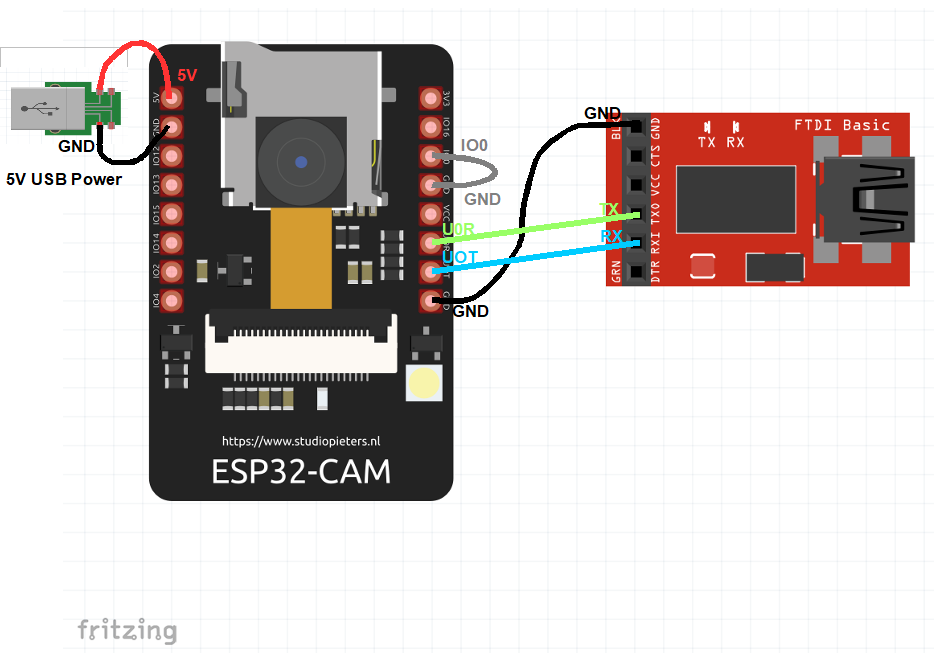
\includegraphics[width=0.80\textwidth]{esp32-cam-s_setup-with_5_usb_power}
\caption[ESP32S CAM setup with external 5V power supply]{ESP32S CAM setup with external 5V power supply \\ Source: own picture}
\label{ESP32-S-CAM-setup-with-external-5v}
\end{figure}